%%%%%%%%%%%%%%%%%%%%%%%%%%%%%% -*- Mode: Latex -*- %%%%%%%%%%%%%%%%%%%%%%%%%%%%
%% 05-10.tex -- Microprocess paper to be submitted for SPW/ProSim 2006
%% Author          : Hongbing Kou
%% Created On      : Mon Sep 23 11:52:28 2002
%% Last Modified By: Philip M. Johnson
%% Last Modified On: Thu Jan 05 10:35:18 2006
%%%%%%%%%%%%%%%%%%%%%%%%%%%%%%%%%%%%%%%%%%%%%%%%%%%%%%%%%%%%%%%%%%%%%%%%%%%%%%%
%%   Copyright (C) 2005 Hongbing Kou
%%%%%%%%%%%%%%%%%%%%%%%%%%%%%%%%%%%%%%%%%%%%%%%%%%%%%%%%%%%%%%%%%%%%%%%%%%%%%%%
%% 

\documentclass[11pt,twocolumn]{article} 
\input{/export/home/csdl/tex/psfig/psfig}
\usepackage{/export/home/csdl/tex/icse2003/latex8}
\usepackage{times}
\usepackage{url}
\usepackage{comment}

%% A verbatim-like environment which allows font changes
%%\usepackage{alltt}
%% New LaTeX2e graphics support
\usepackage[final]{graphicx}
% uncomment the % away on next line to produce the final camera-ready version
% and uncomment the \thispagestyle{empty} following \maketitle
%\pagestyle{empty}
\begin{document}

\title{Automation of Test-Driven Development Validation with Software Microprocess}
\author{
Hongbing Kou and Philip M. Johnson\\
\em  Collaborative Software Development Laboratory \\
\em  Department of Information and Computer Sciences \\
\em  University of Hawai'i \\
\em  [hongbing, johnson]@hawaii.edu}
\maketitle
\thispagestyle{empty}

\begin{abstract}  % 200 words
  Test-Driven Development (TDD) is incremental and iterative with small
  steps in stoplight pattern. This simple principle implies high
  disciplines during software development and there is no effective method
  to validate TDD process so far. We designed and implemented Zorro system
  to automatically examine the microprocesses of TDD with rule-based system
  support. A pilot study is conducted in the University of Hawaii to study
  how and to what extent Zorro can understand and validate TDD
  microprocess, the red/green/refactor iteration.
\end{abstract}

\Section{Introduction}
\label{sec:intro}
Software development is a very complicated process from requirement
analysis through deployment. Traditionally this process is big and heavy,
it is modeled as waterfall model, incremental process model, evolutionary
process model or unified process \cite{Pressman:03}. Agile alliance panel
brought up agile processes to uncover better ways to develop software by
embracing individual and interactions, maintaining always working software,
constantly collaborating with customers and responding to changes in the
development process\cite{AgileAlliance}.  How an individual developer or a
team implements software system becomes more interesting with the birth of
agile processes along with Personal Software Process(PSP) and Team Software
Process(TSP) \cite{Humphrey:99}.

Developers and software institutes may dedicate to well-defined software
processes, or may customize software processes, or may develop software in
ad-hoc manner. The execution of software process largely depends on process
management and self-discipline. It is hard to measure the use of a
particular software process\cite{Janzen:05}, not mention to study how well
processes are complied in a software organization. In the case studies and
experiments of software processes, researchers often used observation or
subjects' oral consensus to ensure process discipline. This manual process
validation is inaccurate and very error-prone. In Collaborative Software
Engineering Laboratory (CSDL) at University of Hawaii, we designed and
implemented Hackystat, an in-process metrics collection system
\cite{csdl2-02-07}. Hackystat automatically collects development activities
and changing metrics of software. With the rich information on development
process, we can reconstruct development process to discover and validate
process execution in software development. We implemented a system called
Zorro on top of Hackystat to automatically discover and validate
Test-Driven Development (TDD), one of the 12 Extreme Programming (XP)
practices. TDD is repetitive and iterative, each iteration starts and ends
with test pass\cite{Beck:03}. In Zorro, we put all kinds of development
activities together to look for the incremental progress made during
software development. It has four components data collection, development
stream construction, microprocess classification and TDD microprocess
validation. The data collection is powered by Hackystat system
\cite{csdl2-02-07} to have in-process development data seamlessly. Zorro
reads in various kinds of development activities to build development
stream; splitting it into TDD microprocesses -- the red/green iterations;
and validate development patterns. Unlike Balboa, we apply the mix of
bottom-up and top-down approaches to study TDD microprocess. By assuming
that developers follow Test-Driven Development principles we present them
in rules to validate the execution process.

Figure \ref{fig:Streaming} is the infrastructure of Zorro system. It
collects development data to make development stream and looks for
development microprocesses with episode identification. In current study we
defined principles of Test-Driven Development as rules in CLIP syntax to
examine development microprocess with JESS rule engine
system\cite{Friedman-Hill:03} support.


\section{Related Work}
\label{sec:related}
Basili commented that ``we have long known that by using standard
engineering and scientific principles, we can improve our profession. What
we have not known is how to introduce these principles in a way that will
convince engineers to consistently practice them.'' \cite{Humphrey:99}
Software process needs discipline and is continuously improved through
``experimentation, measurement and feedback''\cite{Humphrey:99}. In big
software organizations, they may hire process experts to record, examine
and improve their software processes. Individuals and small software teams
are not likely able to afford the process improvement cost as big
organizations do so they will have to conduct experiment, measurement and
process evaluation by themselves. In PSP and TSP, developers record
activity and defect log for process improvement. A pilot study of TSP in
Microsoft found that defect rate is dropped from 25 defects/KLOC to about 7
defects/KLOC\cite{MicrosoftTSP} after adopting TSP. However, the problem is
that developers have to stop their on-hand work frequently to record log
data with PSP/TSP, which brings lots of overhead to developers and software
teams.  Johnson worded that ``You can't even ask them to push a
button.''\cite{csdl2-01-12} to state the urgency to have automatic data
collection tool. Even developers are willing to regularly collect data
manually, it is still not enough. Disney and Johnson found various kinds of
problems in manually entered PSP data\cite{Disney98a}, which have great
impacts on PSP analyses.

The recent trend in software process is agile process, which advocates
incremental iterative development with rapid feedback. Extreme programming
\cite{Beck:00}, one kind of agile process, has 12 practices on planning,
designing, coding and testing. Among these practices, Test-Driven
Development (TDD) is the most well-known one that is being widely
discussed\cite{TddYahooGroup}, supported\cite{Junit,HttpUnit,MockObject},
practiced\cite{TestDrivenWeb,GaryPollice:03,ObjectMentorTDD} and
studied\cite{Muller:02,George:04,Olan:03,Edwards:04}. TDD is incremental
and iterative. In a TDD microprocess, developers \cite{Beck:03}:
\begin{itemize}
\item {Quickly add a test.}
\item {Run all tests and see the new one fail.}
\item {Make a little change.}
\item {Run all tests and see them all succeed.}
\item {Refactor to remove duplication.}
\end{itemize}

There are many case studies on Test-Driven Development. George et al. found
that TDD developers produced higher quality code \cite{George:04} than
controlled groups while M\"uller et al concluded TDD does not accelerate
the implementation and improve the product quality \cite{Muller:02}. Other
studies drew either positive \cite{Olan:03,Edwards:04}, neutral
\cite{Geras:04} or negative \cite{Matjaz:03} conclusion on quality and
productivity of TDD. In the experiments, researchers gave tutorial and
guidelines of Test-Driven Development to test subjects and asked them to
follow guidelines in their development process, final projects are
collected for comparisons against projects developed by controlled groups.
The drawback of this research method is apparent on the fact that Test-Drive
Development has high discipline requirement. The experiment controls are
not good enough to ensure that the stoplight development
pattern\cite{StopLight} of TDD is followed. George et al. stated that one
limitation of their experiment is that test subjects had limited training
on TDD and pair-programming\cite{George:04}, and this problem exists in all
case studies.

Process automation is to build process model out of activity data for
process discovery, validation and improvement. Cook \& Wolf\cite{Cook:95}
developed Balboa to collect development event data with finite state
machine (FSM) to discover the existence of ISPW 6/7 formal software
process. Their work is the complement to process planning and has the
potential to be used for process improvement. Jensen \&
Scacchi\cite{Jensen:04} studied requirements and release process of open
source project NetBeans by analyzing community activities and describing
the process in PML to study the release process execution. Their work
emphasizes on software process from macro point of view and it is often
neglected how developers implement software substantially. The problem in
personal software process and agile process studies is that it relies on
individual's self control and discipline \cite{Humphrey:99}. With our work
we propose and implement a framework to study the microprocess of software
development.  Zorro system is the implementation of this framework
developed with rule-based system support.

\section{Software Development Stream Analysis Framework}
\label{sec:framework}
Software development stream analysis (SDSA) is designed on the rational of
iterative incremental development (IID), that is to say, it is for
microprocess. SDSA framework contains four components data collection,
development stream construction, microprocess tokenization, and
microprocess classification or evaluation. 

\subsection{Data Collection}
SDSA is built on top of Hackystat and it uses service provided by
Hackystat\cite{csdl2-02-07} sensors to collect in-depth development
activities such as file edit, compilation, unit test invocation,
refactoring and debug. SDSA reads in software metric data collected by
Hackystat sensors and derives development actions out of them.

\subsection{Development Stream Construction}
Hackystat defines sensor data type (SDT) to abstract metric data collected
by sensors. We derive development actions by checking the changes of
software metrics and the continuous actions merge together to form 
development stream.
\begin{figure}[ht] 
  \centering
  \includegraphics[width=0.5\textwidth]{picture/Streaming.eps}
  \caption{Development Stream Construction}\label{fig:Streaming}
\end{figure} 

Figure \ref{fig:Streaming} depicts the conceptual structure of development
activity streaming of SDSA. It ends up with development activity stream,
which is very similar to time-series or real-time data.

\subsection{Microprocess Tokenization}
Cook \cite{Cook:95} and Jensen \cite{Jensen:04} studied development stream
with finite state machine (FSM) and PML respectively. Nowadays, software
development is incremental and iterative, we could and probably should
divide development streams into microprocesses to study modern software
development process. Depends on what software processes are employed, there
are many ways to tokenize the development stream into microprocesses. In
our explorative study we introduce \textit{commit tokenizer}, which marks
the end of one iteration with commits to version control system, and
\textit{test-pass tokenizer} is designed to reflect the rhythm of
Test-Driven Development. In situation that one tokenizer is not good
enough, SDSA allows the combination of multiple tokenizers.

\subsection{Microprocess Classification and Evaluation}
In microprocesses, developers conduct development activities following
certain methodology so we will be able to find repetitive patterns. In
stead of looking for patterns in the microprocesses SDSA employs top-down
method to classify and evaluate software microprocess. Knowledge of
development methodology is represented in \textit{if...then...} rules with
rule-engine support to look for matched patterns. Figure
\ref{fig:Classification} illustrates how to apply rules on microprocess
activities.
\begin{figure}[ht] 
  \centering
  \includegraphics[width=0.5\textwidth]{picture/Classification.eps}
  \caption{Microprocess Classification System}\label{fig:Classification}
\end{figure} 

\subsection{Test-Driven Development}
In Test-Driven Development (TDD), Developers write failed test first before
production code. Implementation is driven by test code and the progress is
incremental \cite{Beck:03}.
\begin{quote}
  Red/Green/Refactor is the mantra of Test-Driven Development. It
  implicates the order of programming. 
  \begin{enumerate}
    \item \textit{Red} -- Write a little test that doesn't work, and perhaps
      doesn't even compile at first.
    \item \textit{Green} -- Make the test work quickly, committing whatever
       sins necessary in the process.
    \item \textit{Refactor} -- Eliminate all the duplication created in merely
       getting the test to work.
\end{enumerate}
\end{quote}

Even though TDD is so simple, there is no better way than pair-programming
and informal verbal confirmation to enforce TDD discipline in TDD research
as we discussed in section \ref{sec:related}. TDD practitioners also do not
know how well they are performing in their software development. We
categorizes Test-Driven Development \textit{test-pass} microprocesses into
\textit{Test-Driven} and \textit{Refactoring} in our study.

\subsubsection{Test-Driven}
In a test-driven episode developer writes a test based on requirement
analysis. The test may not even compile at first because the test target
does not exist yet. There should have compilation failure if developer
compiles it or project was configured to be compiled automatically.
Production code is created to get rid of compilation error.  Execution of
this test will probably fail when developer invokes it, which is the red
bar pattern. The rest work of this episode is to have just enough code to
make test pass. This is the scenario of a typical test-driven episode. Even
though developers can be required to follow typical test-driven strictly it
is lame to have this discipline requirement. In some cases there is no
point to let developer do it rigiously.
\begin{itemize}
\item Test code compilation will definitely fail because it tests
  non-existed object or method.
\item The production code to make test pass is trivial. Generating a fake
  implementation to make test fail will be just a waste.
\end{itemize}

The key to TDD is the test case creation and the substantial work to make
test pass. They are the skeleton of a test-driven episode. Depending on the
existence of compilation error and test failure, a test-driven episode can
be one of them in figure \ref{fig:Test-Driven}.

\begin{figure}[ht] 
  \centering
  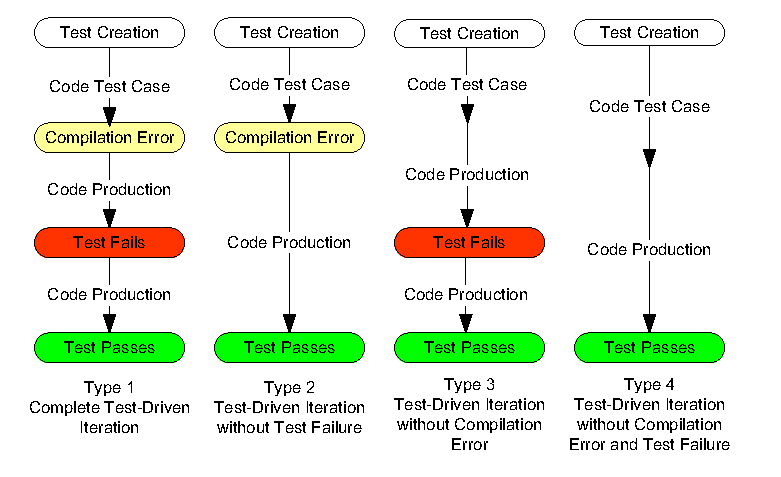
\includegraphics[width=0.5\textwidth]{picture/TDD-Microprocess.eps}
  \caption{Test-Driven Microprocess}\label{fig:Test-Driven}
\end{figure}

\subsubsection{Refactoring}
Refactoring is the term describes operation to alter a program's internal
structure without changing its external behaviors in software development
\cite{Refactoring}. New feature is introduced by new test cases in TDD such
that a test-pass microprocess is refactoring as long there is no new test.
Refactoring episode also has four types. In one side refactor can happen
either to test code or production. On another side refactoring operation
may or may not fail the existed tests. Figure \ref{fig:Refactoring} depicts
the algorithm of this categorization. In types 3 and 4 there may have some
work on test code without new test created.

\begin{figure}[ht] 
  \centering
  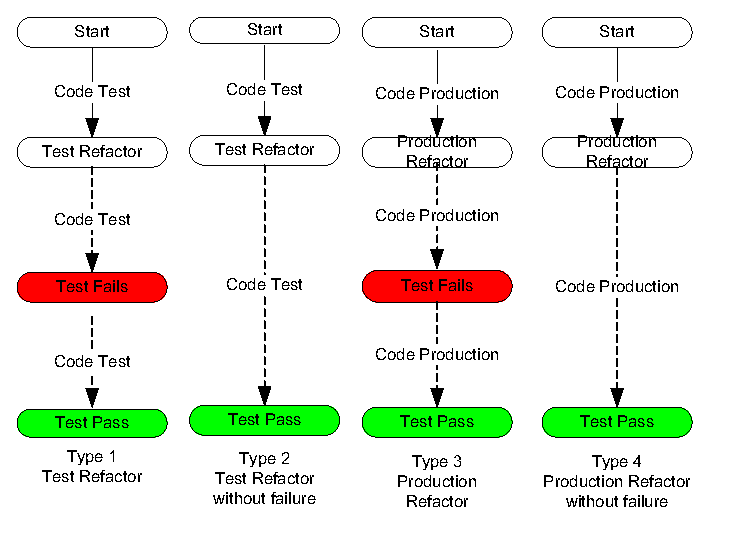
\includegraphics[width=0.5\textwidth]{picture/Refactoring-Microprocess.eps}
  \caption{Refactoring Microprocess}\label{fig:Refactoring}
\end{figure} 

\subsubsection{Test-Last and Validation}
Ideally a test-pass microprocess is either test-driven or refactoring in
Test-Driven Development. The allowance is that developer may create
multiple test cases for the production code to test various inputs. We call
this Test-Last Development contrary to Test-Driven Development in that test
code is created after production code. It is also the canonical programming
habit of most non-TDD developers. Regression or validation is to run the
existed tests to make sure system work well without changing anything,
which happens very often in software development. 

\section{A Case Study on Test-Driven Development}
\label{sec:casestudy}
The Software Development Stream Analysis (SDSA) framework views software
development from micro-level to support both \textit{in vivo} and \textit{in
  vitro} empirical software process study. Zorro system is our
implementation of this framework to explore its capability on evaluating
Test-Driven Development in particular. To study how and to what extent we
can automate the TDD evaluation in software development, we conducted a
case study at a software engineering research lab in University of Hawaii.

\subsection{Experiment Setup}
We required test subjects have substantial knowledge of Java programming
language and good understanding of unit tests. Eclipse IDE is the
development platform we currently have comprehensive sensor support so we
asked subjects use Eclipse and install Hackystat Eclipse sensor
\cite{HackystatSensor} before the experiment. We observed subject's
programming activities and recorded them to compare our observation with
the evaluated results from Zorro.

\subsection{Tutorial and Guideline}
In the experiment we provided a brief introduction and gave instructive
guideline on how to implement a stack data structure in Test-Drive
Development fashion. Stack is an essential data structure and requirements
to stack is well-known to computer science students. 

\section{Lessons Learned and Discussion}
\label{sec:discussion}

\bibliographystyle{/export/home/csdl/tex/icse2003/latex8}
\bibliography{/export/home/csdl/bib/zorro,/export/home/csdl/bib/tdd,/export/home/csdl/bib/csdl-trs,/export/home/csdl/bib/hackystat,/export/home/csdl/bib/psp}
\end{document}











